\documentclass[12pt,a4paper]{amsart}
\usepackage[a4paper,margin=1in]{geometry}
\usepackage[euler-digits]{eulervm}
\usepackage{tikz}
\usetikzlibrary{calc}

\begin{document}
\section*{$C_7$.}
\begin{center}
  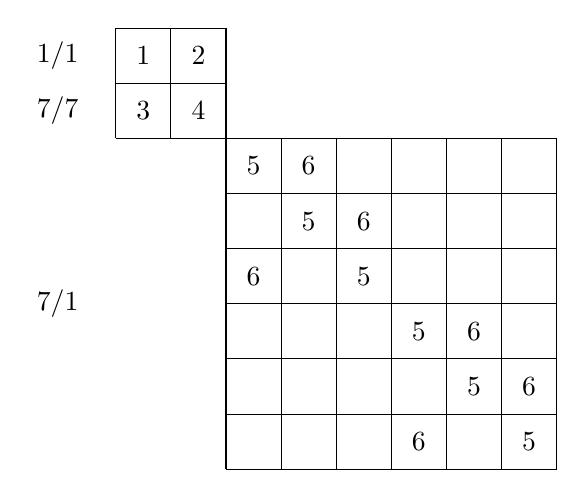
\begin{tikzpicture}[xscale=0.7,yscale=-0.7]
    \draw[shift={(0.5,0.5)}](0,0) grid (2,2);
    \draw[shift={(0.5,0.5)}](2,2) grid (8,8);
    \node[anchor=east] at (0,1) {$1/1$};
    \node[anchor=east] at (0,2) {$7/7$};
    \node[anchor=east] at (0,5.5) {$7/1$};
    \foreach \i in {1,...,4}
      \node[anchor=center] at ({mod(\i-1,2)+1}, {int((\i+1)/2)}) {$\i$};
    \node[anchor=center] at (3, 3) {$5$};
    \node[anchor=center] at (4, 4) {$5$};
    \node[anchor=center] at (5, 5) {$5$};
    \node[anchor=center] at (6, 6) {$5$};
    \node[anchor=center] at (7, 7) {$5$};
    \node[anchor=center] at (8, 8) {$5$};
    \node[anchor=center] at (3, 5) {$6$};
    \node[anchor=center] at (4, 3) {$6$};
    \node[anchor=center] at (5, 4) {$6$};
    \node[anchor=center] at (6, 8) {$6$};
    \node[anchor=center] at (7, 6) {$6$};
    \node[anchor=center] at (8, 7) {$6$};
      \end{tikzpicture}
%\end{center}
\quad
%\begin{center}
  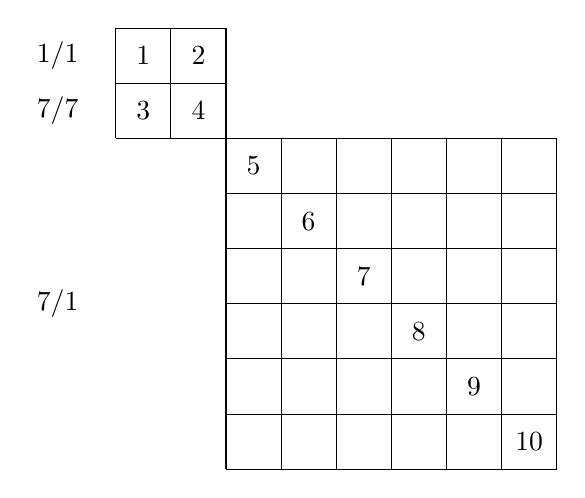
\begin{tikzpicture}[xscale=0.7,yscale=-0.7]
    \draw[shift={(0.5,0.5)}](0,0) grid (2,2);
    \draw[shift={(0.5,0.5)}](2,2) grid (8,8);
    \node[anchor=east] at (0,1) {$1/1$};
    \node[anchor=east] at (0,2) {$7/7$};
    \node[anchor=east] at (0,5.5) {$7/1$};
    \foreach \i in {1,...,4}
      \node[anchor=center] at ({mod(\i-1,2)+1}, {int((\i+1)/2)}) {$\i$};
    \node[anchor=center] at (3, 3) {$5$};
    \node[anchor=center] at (4, 4) {$6$};
    \node[anchor=center] at (5, 5) {$7$};
    \node[anchor=center] at (6, 6) {$8$};
    \node[anchor=center] at (7, 7) {$9$};
    \node[anchor=center] at (8, 8) {$10$};
      \end{tikzpicture}
\end{center}


\end{document}
